\documentclass[11pt, oneside, fullpage, doublespace]{article}
\usepackage{geometry}                		% See geometry.pdf to learn the layout options. There are lots.
\geometry{letterpaper}                   		% ... or a4paper or a5paper or ... 
%\geometry{landscape}                		% Activa te for for rotated page geometry
%\usepackage[parfill]{parskip}    		% Activate to begin paragraphs with an empty line rather than an indent
\usepackage{graphicx}				% Use pdf, png, jpg, or eps� with pdflatex; use eps in DVI mode
								% TeX will automatically convert eps --> pdf in pdflatex	
\usepackage{amssymb}
\usepackage{hyperref}
\usepackage{color}

\usepackage{setspace}
\setstretch{1.5}
\usepackage{enumerate}
\usepackage{paralist}


% Code formatting
\usepackage{listings}
\usepackage{color}
\definecolor{mygreen}{rgb}{0,0.6,0}
\definecolor{mygray}{rgb}{0.5,0.5,0.5}
\definecolor{mymauve}{rgb}{0.58,0,0.82}
\lstset{ %
  backgroundcolor=\color{white},   % choose the background color
  basicstyle=\footnotesize\ttfamily,        % size of fonts used for the code
  breaklines=true,                 % automatic line breaking only at whitespace
  captionpos=b,                    % sets the caption-position to bottom
  commentstyle=\color{mygreen},    % comment style
  escapeinside={\%*}{*)},          % if you want to add LaTeX within your code
  keywordstyle=\color{blue},       % keyword style
  stringstyle=\color{mymauve},     % string literal style
}



\title{Cell Tower Population Estimation Through the Use of Voronoi Tessellations}
\author{Santiago Gonzalez\\ \emph{Undergraduate, EECS Department, Colorado School of Mines}}
\date{May 6, 2014}


\begin{document}
\maketitle

\begin{abstract} 
This paper describes a system in which populations surrounding cell towers can easily be estimated. The system is designed with the objective that result data could be used to improve human mobility models. The project was conducted as a two credit-hour independent study for the computer science PhD student, Thyago Mota, to assist with his mobility model research at the Colorado School of Mines. The population estimation system operates by partitioning a geographic area into various segments, surrounding a provided set of cell tower coordinates, using a Voronoi tessellation. This generated tessellation is used in conjunction with NASA's large Gridded Population of the World dataset, which provides population estimates for the entire world on an approximately five kilometer square grid, to return a per cell tower population estimate. The system relies on efficient programing due to the large size of the datasets being utilized. To accomplish the system's objectives, a solution was implemented as a collection of programs written in JavaScript, Ruby, and Python. Results and potential improvements to the system are also discussed.
\end{abstract}

\section{Introduction}
The development of human mobility models has been an area of intense research over the past several years. Human mobility models have a wide variety of applications, including improved automation, occupancy prediction, and improved public transportation network design. Recently, cell tower log data has been utilized to gain new insight into human mobility models with high temporal accuracy. Such models could be improved by having set estimates of populations surrounding each cell tower.

This project aims to accurately estimate cell tower surrounding populations using cell tower locations as inputs and NASA's Gridded Population of the World dataset. A Voronoi tessellation is run on the input location data to segment a geographic area into various polygons, each of which has a cell tower at its center. Such a Voronoi tessellation is a good representation of the distribution of people per cell tower since each edge within a polygon is inherently an orthogonal bisector of the line between two cell towers.

Overall, the system appears to function adequately. However, there are several improvements that can be introduced into the system to improve performance due to the highly parallelizable nature of the estimation problem. Future research in this area will involve comparison of this system's results with population estimates gathered from call log data and population estimates from Twitter to evaluate each method's efficacy.

\section{Related Work}
\cite{motahari2012} describes a framework for estimating wireless subscriber populations within cellular carriers using a pattern regularity-based system. Such a system provides data that can help to improve urban mobility models. The researchers were able to test the system on CDMA EV-DO cellular data usage data and resulted in high-accuracy subscriber estimations.

\cite{csis} discusses research on urban mobility models using population estimates that are calculated from call log data. The researchers claim that better understanding of urban mobility models would improve city planning and public space management. Identifying call patterns and general activity patterns with high temporal and spacial resolution would permit dynamic population estimation at any given point in time. The produced estimates were found to concur with actual, measured populations.

\subsection{Gridded Population of the World}
\begin{figure}
\begin{center}
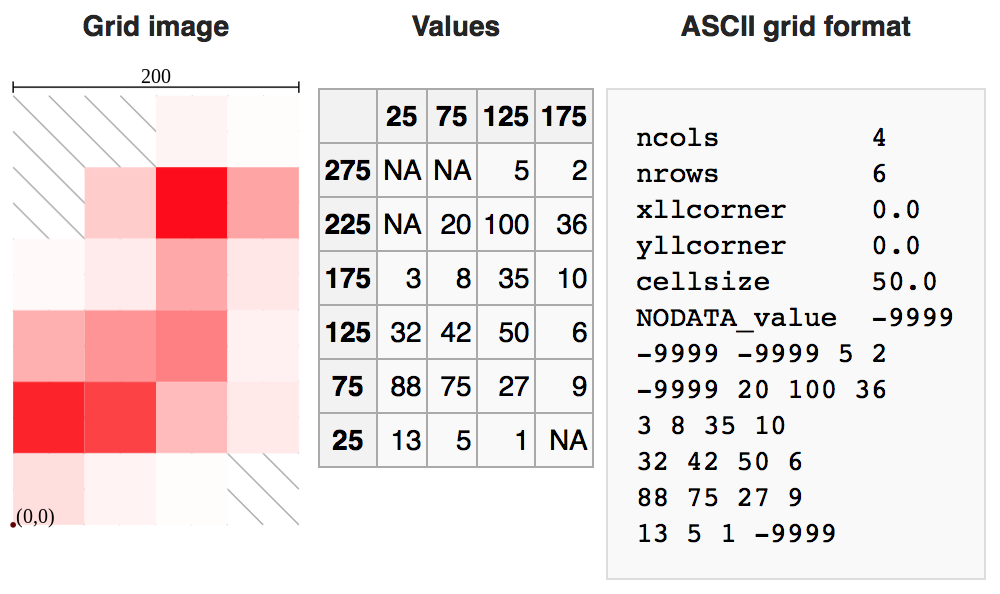
\includegraphics[width=3.5in]{esri}
\end{center}
\caption{Esri ASCII Raster Format -- from \cite{esri}}
\label{fig:esri}
\end{figure}
The NASA Socioeconomic Data and Applications Center (SEDAC) has developed a global population distribution dataset, named Gridded Population of the World version 3 (GPW) \cite{gpw}. GPW provides a representation of the world's population count, set on 2.5 arc-minute square grid (translating to an approximately five kilometer square grid at the equator). GPW data is provided as an Esri raster file, detailed in Figure \ref{fig:esri}.  This dataset was generated using a proportional allocation gridding algorithm to assign cell values within the grid. The 2010 GPW dataset has been utilized in this project as a granular population data source.


\section{Project Overview and Methods}

\begin{figure}
\begin{center}
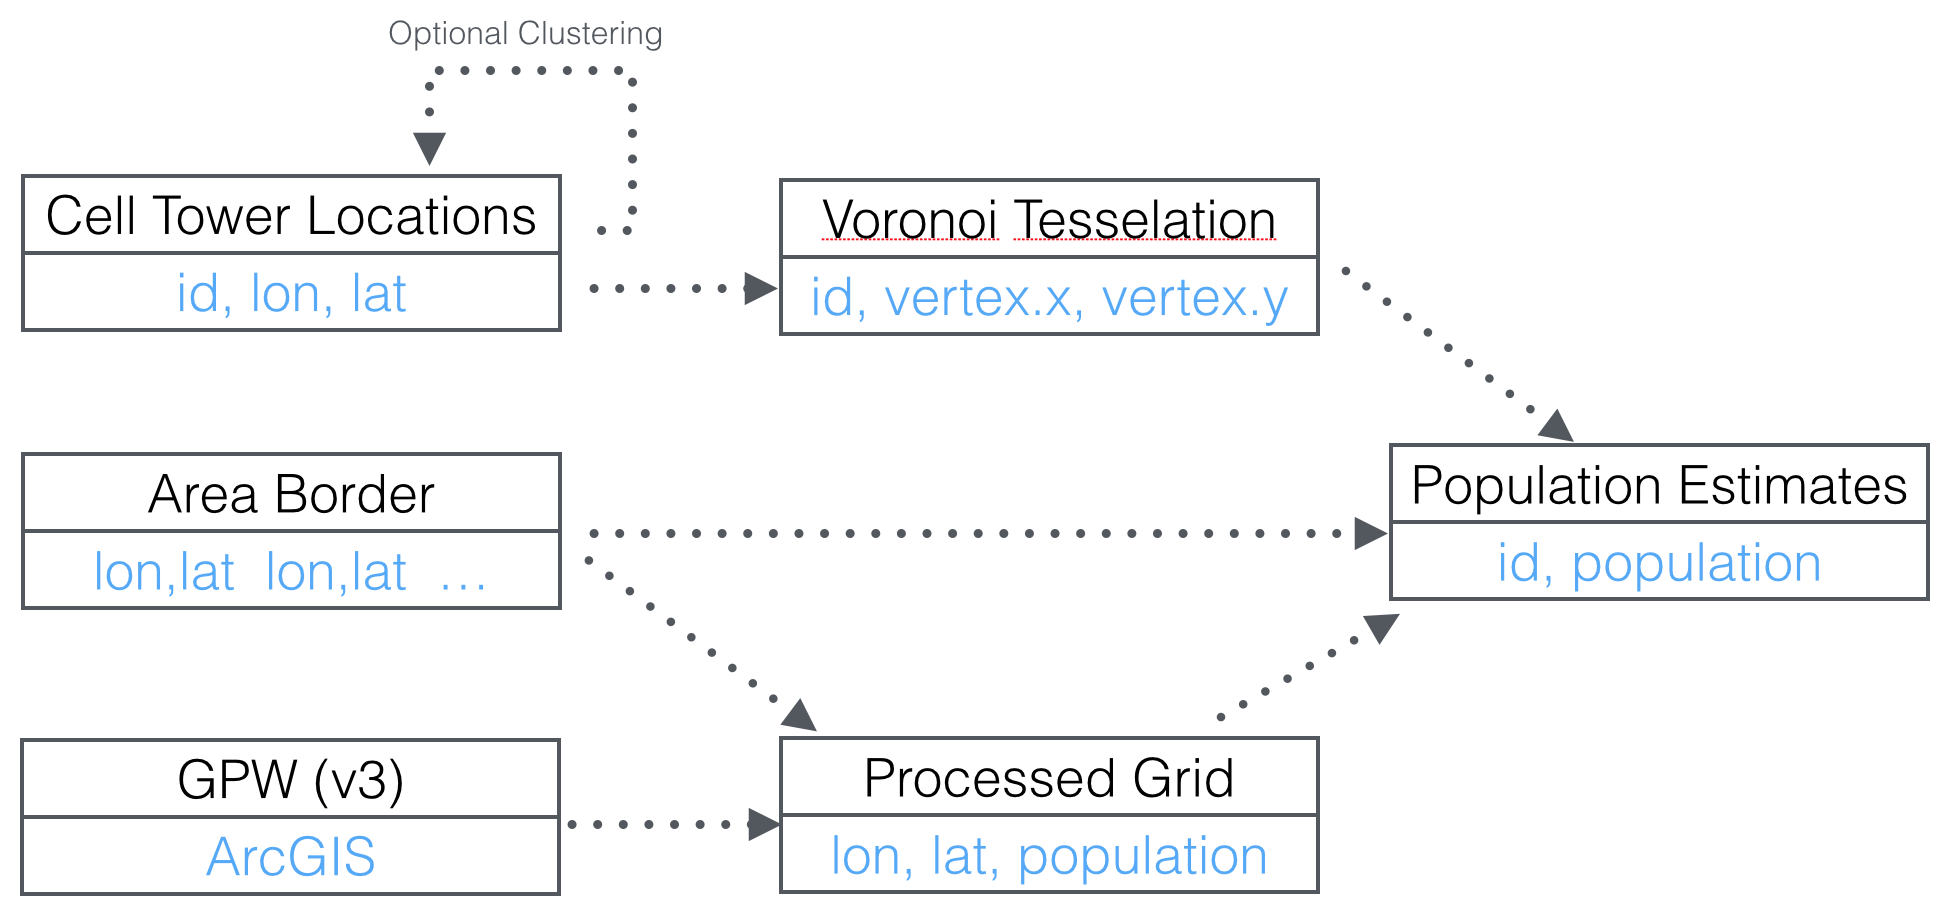
\includegraphics[width=6in]{architecture}
\end{center}
\caption{High-Level System Overview}
\label{fig:system}
\end{figure}

The project described in this paper has been broken into various pieces to improve manageability. Figure \ref{fig:system} shows the overall architecture and flow of data within the system. The system relies on three main components:
\begin{enumerate}
\item GPW Processing Scripts, 
\item Voronoi Tessellation, and
\item Population Estimator.
\end{enumerate}


\subsection{Datasets}
Two empirical datasets were chosen for this project: An Ivory Coast dataset consisting of 1238 cell tower locations, and an Abidjan dataset consisting of 383 cell tower locations, a small subset of the Ivory Coast dataset that focusses around its largest city, Abidjan. The Ivory Coast was chosen due to the free availability of cell tower information, which is inaccessible within the United States.

\subsection{Gridded Population of the World Processing}
Substantial processing is performed on the GPW data prior to use within the estimation program using a Python script with the $\texttt{shapely}$ module. The Esri grid format metadata (Figure \ref{fig:esri}) is first read from the GPW datafile. In conjunction with an outline geometry file, data is extracted from the GPW file and output to a CSV file in longitude, latitude, population format. This processing removes unnecessary, outlying data points from the GPW data, ultimately reducing the 1.3GB Ivory Coast GPW raster file to an easily parsable, 780MB CSV file.


\subsection{Voronoi Tessellation}
\begin{figure}
\begin{center}
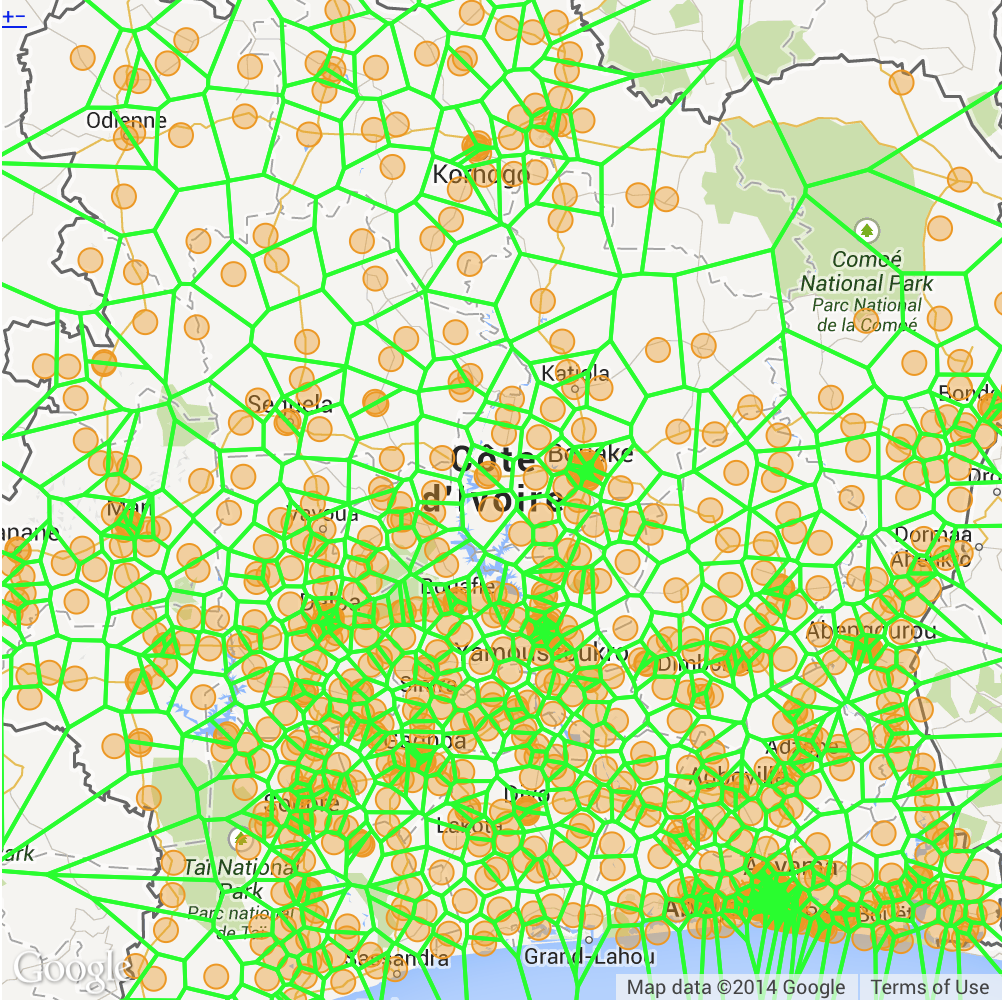
\includegraphics[width=4in]{ivorycoastvoronoi}
\end{center}
\caption{Voronoi Tessellation for Ivory Coast Dataset}
\label{fig:ivorycoastvoronoi}
\end{figure}

\begin{figure}
\begin{center}
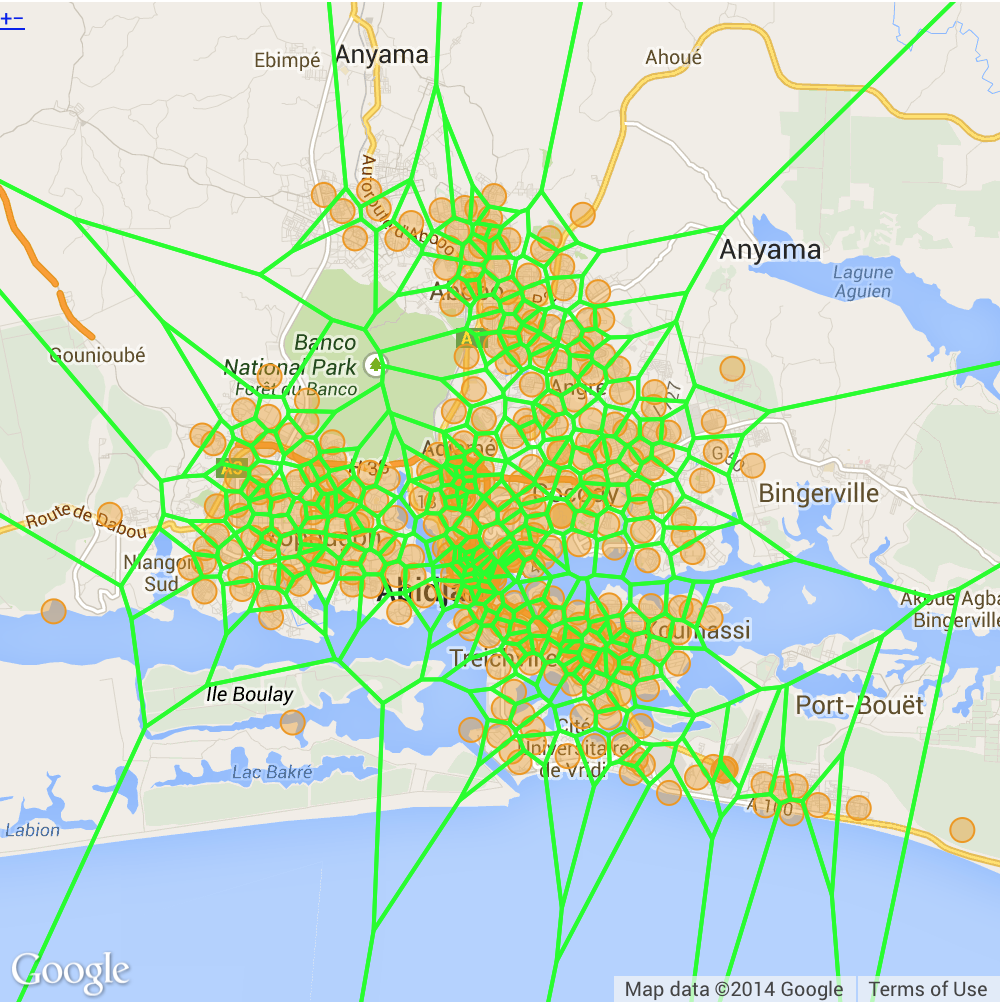
\includegraphics[width=4in]{abidjanvoronoi}
\end{center}
\caption{Voronoi Tessellation for Abidjan Dataset}
\label{fig:abidjanvoronoi}
\end{figure}

A Voronoi tessellation is a method of dividing an n-dimensional space, such as a plane, into various regions, such as polygons, around a set of center-points. Every point in each region is closest to that region's corresponding center-point. The Voronoi tessellation for a set of points is inverse to the Delaunay triangulation for that same set of points. For this project we shall consider a two-dimensional Voronoi tessellation. Using a Voronoi tessellation is logical since each polygon's corresponding cell tower is the cell tower with the strongest signal within that polygon, assuming homogeneous cell towers.

The JavaScript Topology Suite (JSTS) \cite{jsts} was selected for this project due to its ease of use, ability to process large sets of points, and integration with OpenLayers \cite{openlayers}. JSTS is a JavaScript implementation of the widely used Java Topology Suite (JTS).

The Voronoi tessellation component of the system is written in JavaScript and utilizes JSTS to calculate the Voronoi polygons for a set of cell tower coordinates which are then overlaid on a Google map using OpenLayers. The Voronoi tessellations for both datasets (Figure \ref{fig:ivorycoastvoronoi} and Figure \ref{fig:abidjanvoronoi}) are calculated quickly, in under one second. The resultant tessellation is output as a plain-text list of identifiers and polygons, each in Well Known Text (WKT) format. This output is then converted into an easily parsable CSV file using regular expressions in a Ruby script.


\subsection{Population Estimation}
Population estimation is implemented using a Python script with the $\texttt{shapely}$ module. The processed GPW CSV file is read into memory along with the Voronoi polygon CSV file and the outline geometry file. A hash-table mapping from cell tower identifier to estimated population is created where all values map to zero. The program then iterates over each GPW population datapoint together with each Voronoi polygon and adds the GPW population to the current cell tower's entry within the hash-table if the GPW population datapoint's latitude and longitude are contained within the Voronoi polygon. Estimates are then output from the hash-table into a CSV file.



\section{Results and Future Research}
The system can run on empirical datasets with results that concur with measured data. The Voronoi tessellation component can be clearly observed to produce correct Voronoi polygons for a set of cell tower coordinate inputs. Upon running the Abidjan dataset through the system, the aggregate population sum was found to be 3,812,122 people (using 2010 GPW data). The population of Abidjan in 2006 was 3,796,677 people \cite{abidjanpop}. The actual and estimated populations are nearly identical, taking population growth and potentially different borders into account.

There is substantial future research that can be performed to add features and improve the performance of this system. Currently, all population estimation tasks are performed on one single thread. Due to the easily parallelizable nature of the estimation algorithm, the population estimation program could be modified to take advantage of the several processor cores available on the host machine to significantly reduce run times.

There is room for substantial future research to determine the validity and usefulness of the generated population estimates. Other population estimation methods, including those produced from analyzing call log data and geotagged tweets from Twitter, can be compared with the method presented in this paper to evaluate each method's effectiveness and applicability to human mobility models.

\section{Summary}
In the hopes of facilitating the improvement of human mobility models, a system has been developed for Colorado School of Mines PhD student, Thyago Mota, that is capable of estimating the populations surrounding cell towers. This system applies a Voronoi tessellation on a set of cell tower coordinate points to segment a local polygon for each datapoint. These Voronoi polygons are then used in conjunction with a Gridded Population of the World dataset and an outline geometry of the region of interest to generate a population estimate for each cell tower.

The system has been applied to an Ivory Coast dataset and an Abidjan dataset, and successfully generates estimates that, when aggregated, appear to be correct. Further research in this area will involve the analysis and comparison of these estimates with additional population estimation methods, including the use of call log data and geotagged Twitter messages.


\begin{thebibliography}{99}
\bibitem{motahari2012} S. Motahari, K. Jintaseranee, P. Reuther, Hui Zang, ``Regularity-based wireless subscriber population estimation,'' \emph{Global Communications Conference (GLOBECOM), 2012 IEEE} , vol., no., pp.5177,5182, 3-7 Dec. 2012

\bibitem{csis} The University of Tokyo, ``A Study on Urban Mobility and Dynamic Population Estimation by Using Aggregate Mobile Phone Sources,'' \emph{Center for Spatial Information Science} [Online]. Available: \url{http://www.csis.u-tokyo.ac.jp/dp/115.pdf}

\bibitem{gpw} NASA Socioeconomic Data and Applications Center (SEDAC), ``Gridded Population of the World (GPW) v3,'' [Online]. Available: \url{http://sedac.ciesin.columbia.edu/data/collection/gpw-v3}

\bibitem{esri} Wikipedia, ``Esri grid,'' [Online]. Available: \url{https://en.wikipedia.org/wiki/Esri_grid}

\bibitem{jsts} Bj�rn Harrtell, ``JavaScript Topology Suite (JSTS),'' \emph{GitHub} [Online]. \url{https://github.com/bjornharrtell/jsts}

\bibitem{openlayers} ``OpenLayers,'' [Online]. \url{http://openlayers.org}

\bibitem{abidjanpop} Princeton Universite, ``Abidjan,'' [Online]. Available: \url{http://www.princeton.edu/~achaney/tmve/wiki100k/docs/Abidjan.html}

\end{thebibliography}


















\section*{Appendix 1 --- Code Listings}
Code relevant to this project has been appended in the following subsections. This code, along with input data, documentation, and a README, is available as a public repository on GitHub at \url{https://github.com/sgonzalez/cell-tower-population}.
\subsection*{Voronoi Tessellation \emph{(abridged)}}
\emph{Input data has been removed from this code listing for brevity.}
\begin{spacing}{1}
\begin{lstlisting}[language=html]
<!DOCTYPE html PUBLIC "-//W3C//DTD XHTML 1.0 Strict//EN" "http://www.w3.org/TR/xhtml1/DTD/xhtml1-strict.dtd">
<html>

<!-- HEAD -->
<head>
	<title>Voronoi Tesselation Example</title>
	<meta http-equiv="Content-Type" content="text/html; charset=utf-8"/>
    <meta name="Author" content="Thyago Mota"/>
</head>

<script src="http://maps.google.com/maps/api/js?sensor=false"></script>
<script type="text/javascript" src="OpenLayers.js"></script>
<script type="text/javascript" src="javascript.util.js"></script>
<script type="text/javascript" src="jsts.js"></script>
<script type="text/javascript" src="attache.array.min.js"></script>
<script type="text/javascript">
	var map, baseLayer, sitesLayer, tilesLayer;

	function init() {
		// 0. the parser object converts objects from JSTS to OpenLayers
		var parser = new jsts.io.OpenLayersParser();

		// 1. these objects will be necessary to convert from one projection to another
		var epsg4326   = new OpenLayers.Projection('EPSG:4326');
		var epsg900913 = new OpenLayers.Projection('EPSG:900913');

		// 2. define the points in JSTS
		var jstsPoints = [
//// INSERTION POINT ////

//// END POINT ////

			/*new jsts.geom.Coordinate(-105.210492, 39.750589),
			new jsts.geom.Coordinate(-105.222601, 39.751347),
			new jsts.geom.Coordinate(-105.153801, 39.736102),
			new jsts.geom.Coordinate(-105.223925, 39.742108)*/
		];

		// 3. calculate the voronoi tesselation
		var geometryFactory = new jsts.geom.GeometryFactory();
		var jstsMultipoints = geometryFactory.createMultiPoint(jstsPoints);
		var voronoiBuilder  = new jsts.triangulate.VoronoiDiagramBuilder();
		voronoiBuilder.setSites(jstsMultipoints);
		var voronoi         = voronoiBuilder.getDiagram(geometryFactory);

		// 4. create an openlayers map
		map = new OpenLayers.Map('map', {projection: "EPSG:900913"});

		// 5. base layer is a google map
		baseLayer = new OpenLayers.Layer.Google('Google Map Layer', {layers: 'basic'});

		// 6. have a layer with the sites
		sitesLayer = new OpenLayers.Layer.Vector('sites layer');
		var features1 = new Array(jstsPoints.length);
		var point;
		for (var i in jstsPoints) {
			point = new OpenLayers.Geometry.Point(jstsPoints[i].x, jstsPoints[i].y);
			features1[i] = new OpenLayers.Feature.Vector(point.transform(epsg4326, epsg900913), null);
		}
		sitesLayer.addFeatures(features1);

		// 7. have another layer with the tiles
		tilesLayer = new OpenLayers.Layer.Vector('tiles layer');
		var geometries = parser.write(voronoi).components;
		var features2 = new Array(geometries.length);
		for (var i in geometries) {
			features2[i] = new OpenLayers.Feature.Vector(geometries[i].transform(epsg4326, epsg900913), null, {fillOpacity:0,strokeColor:'#00FF00'});
		}
		tilesLayer.addFeatures(features2);

		// 8. add the layers to the map
		map.addLayers([baseLayer, sitesLayer, tilesLayer]);

		// 9. do the zoom
		map.zoomToExtent(tilesLayer.getDataExtent());



		var button = document.getElementById('exportButton');
        button.addEventListener('click', exportToCsv);

        function exportToCsv() {
            var myCsv = "";

//    		myCsv += voronoi;
            // var pointIndex = 1;
            // var voronoiResult = voronoiBuilder.getDiagram(geomFact);
            // var parser = new jsts.io.OpenLayersParser();
            // input = parser.write(input);
            // voronoiResult = parser.write(voronoiResult);
            // vertices = voronoiResult.getVertices();
			/*var str = '';
			for (i in vertices) {
				point = vertices[i];
				point = point.transform(epsg900913,epsg4326);
				str = str + point.x + ',' + point.y + ' ';
				str += '\n'
			}*/
            var gs = parser.write(voronoi).components;
            var pointIndex = 1;
            for (var i in gs) {
                var verts = gs[i]/*.transform(epsg900913, epsg4326)/*.transform(epsg4326, epsg900913)*/.getVertices();
                myCsv += pointIndex;
                myCsv += " ";
                myCsv += verts;
                myCsv += "\n";
                /*for (var loc in verts) {
                    myCsv += loc instanceof OpenLayers.Geometry;
                    myCsv += "     ";
                    myCsv += pointIndex;
                    myCsv += ", ";
                    myCsv += loc.latitude;
                    myCsv += ", ";
                    myCsv += loc.longitude;
                    myCsv += "\n";
                }*/
                pointIndex ++;
                // features2[i] = new OpenLayers.Feature.Vector(geometries[i].transform(epsg4326, epsg900913), null, {fillOpacity:0,strokeColor:'#00FF00'});
            }
//            var vtcs = voronoi.getCoordinates();
//    		var str = '';
//    		var p;
//    		for (i in vtcs) {
//    			p = vtcs[i];
//                // p = p.transform(epsg900913,epsg4326);
//    			str = str + p.x + ',' + p.y + '\n';
//    		}
//            myCsv += str;
            // var resultString = '';
            // var index = 0;
            // for (i in voronoi.getVertices()) {
            //     resultString += index;
            //     index++;
            // }
            // myCsv += voronoi.getCoordinates();

    		/*for (var pt in jstsPoints) {
    		    for (var i in g) {
        			f[i] = new OpenLayers.Feature.Vector(g[i].transform(epsg4326, epsg900913), null, {fillOpacity:0,strokeColor:'#00FF00'});
        			myCsv += f[i];

        			myCsv += pointIndex;
        		    myCsv += ", ";
        		    myCsv += pt.latitude;
        		    myCsv += ", ";
        		    myCsv += pt.longitude;
        		    myCsv += "\n";
        		}
    		    pointIndex++;
    		}*/

            window.open('data:text/csv;charset=utf-8,' + escape(myCsv));
        }
	}
</script>

<!-- BODY -->
<body onload="init()">
	<div id="map" style="width: 500px; height: 500px;"></div>
	<P>
	<!--<textarea id="text" rows="20" cols="50"></textarea>-->
	<button id="exportButton">Export Geometries to CSV</button>
</body>

</html>

\end{lstlisting}
\end{spacing}

\subsection*{Voronoi WKT to CSV Converter}
\begin{spacing}{1}
\begin{lstlisting}[language=ruby]
#!/usr/bin/ruby

#########################
### Santiago Gonzalez ###
#########################

def process_line line, poly_out_file, pops_out_file
  split_line = line.split(' ', 2)
  polygon_id = split_line[0]
  points = split_line[1].scan(/POINT\((-?\d+\.\d+) (-?\d+\.\d+)\)/)

  points.each do |vertex|
    print polygon_id
    print ", "
    print vertex[0]
    print ", "
    print vertex[1]
    puts ""
    poly_out_file.write("#{polygon_id}, #{vertex[0]}, #{vertex[1]}\n")
  end
  
  puts ""
end


############################
## PROGRAM EXECUTION START

# take input file argument
if ARGV.length != 1
  puts "Usage: ./polygon_processor.rb [results file]"
  exit 1
end
filename = ARGV[0]

# parse file line by line
File.open(filename, "r") do |file|
  File.open("OUTPUT/parsed_polygons.csv", 'w+') do |poly_out_file|
    File.open("OUTPUT/polygon_populations.csv", 'w') do |pops_out_file|
      file.each do |ln|
        process_line ln, poly_out_file, pops_out_file
      end
    end
  end
end

exit 0

\end{lstlisting}
\end{spacing}

\subsection*{Grid Converter}
\begin{spacing}{1}
\begin{lstlisting}[language=python]
# ------------------------------------------------------------------------------- #
# grid_converter.py - Converts a grid map with population to the following format #
# lon, lat, population                                                            #
# Author: Thyago Mota                                                             #
# Date: 02/01/2014                                                                #
# ------------------------------------------------------------------------------- #

import datetime, shapely, sys, math
from datetime import datetime, date, time
from shapely.geometry import Polygon, Point
from math import modf

def help():
	print('Use: ' + sys.argv[0] + ' input_file geometry_file output_file')

# ------------------------------------------------------------------------------- #
# Some definitions                                                                #
# ------------------------------------------------------------------------------- #
FEEDBACK_NUM_RECORDS = 100
NUM_ARGS             = 4
TOLERANCE            = 0.00001
ARCGIS_NO_DATA_VALUE = -3.40282346639e+038

# ------------------------------------------------------------------------------- #
# Script begins                                                                   #
# ------------------------------------------------------------------------------- #
startTime = datetime.now()
print('Start time: ' + str(startTime.hour) + ':' + str(startTime.minute) + ':' + str(startTime.second)) 

# ------------------------------------------------------------------------------- #
# Command line validation                                                         #
# Parameters (required): input_file output_file                                   # 
# ------------------------------------------------------------------------------- #
if len(sys.argv) != NUM_ARGS:
	help()
	exit(1)
	
# ------------------------------------------------------------------------------- #
# Opening of files                                                                #
# ------------------------------------------------------------------------------- #
print('Trying to open the input and geometry files for reading')
try: 
	input = open(sys.argv[1], 'rt')
except:
	print('Could not open file ' + sys.argv[1])
	exit(2)
try: 
	geometry = open(sys.argv[2], 'rt')
except:
	print('Could not open file ' + sys.argv[2])
	input.close()
	exit(3)
try: 
	output = open(sys.argv[3], 'wt')
except:
	print('Could not open file ' + sys.argv[3])
	input.close()
	geometry.close()
	exit(4)
print('Success!')

# ------------------------------------------------------------------------------- #
# Reading geometry file                                                           #
# ------------------------------------------------------------------------------- #
print('Reading geometry file')
geoData = []
for line in geometry:
	line = line.replace('\n', '')	
	data = line.split(' ')
	for i in range(0, len(data)):
		d = data[i].split(',')
		geoData.append([float(d[0]), float(d[1])])
geometry.close()
print('Geometry file looking good :-)')
#print(geoData)

# ------------------------------------------------------------------------------- #
# Creating a polygon based on geometry                                            #
# ------------------------------------------------------------------------------- #
print('Creating a polygon based on geometry')
poly = Polygon(geoData)
print('That was easy!')

# ------------------------------------------------------------------------------- #
# Reading metadata                                                                #
# ------------------------------------------------------------------------------- #
print('Metadata:')
for i in range(0, 6):
	line = input.readline()
	line = line.replace('\n', '')
	line = " ".join(line.split()) # eliminates duplicate whitespaces
	data = line.split(' ')
	#print(data[1])
	if i == 0:
		nCols = int(data[1])
	elif i == 1:
		nRows = int(data[1])
	elif i == 2:
		xllCorner = float(data[1])
	elif i == 3:
		yllCorner = float(data[1])
	elif i == 4:
		cellSize = float(data[1])
	else:
		noDataValue = float(data[1])
print('\tnCols: \t\t' + str(nCols))
print('\tRows: \t\t' + str(nRows))
print('\txllCorner: \t' + str(xllCorner))
print('\tyllCorner: \t' + str(yllCorner))
print('\tcellSize: \t' + str(cellSize))
print('\tnoDataValue: \t' + str(noDataValue))
print('Grid box:')
print('\t(' + str(xllCorner) + ',' + str(yllCorner) + ')')
print('\t(' + str(xllCorner + nCols * cellSize) + ',' + str(yllCorner) + ')')
print('\t(' + str(xllCorner) + ',' + str(yllCorner + nRows * cellSize) + ')')
print('\t(' + str(xllCorner + nCols * cellSize) + ',' + str(yllCorner + nRows * cellSize) + ')')

# ------------------------------------------------------------------------------- #
# Reading the grid                                                                #
# ------------------------------------------------------------------------------- #
grid = [ [ 0. for j in xrange(nCols) ] for i in xrange(nRows) ]
i = 0
totalUnbounded = 0
for line in input:
	line = line.replace('\n', '')
	if line[0] == ' ':
		line = line[1:]
	data = line.split(' ')
	for j in xrange(nCols):
		value = float(data[j])
		if value == ARCGIS_NO_DATA_VALUE or value == noDataValue or value < 0:
			continue
		grid[i][j] = value
		totalUnbounded = totalUnbounded + value
	i = i + 1
input.close()
print('Total unbounded: ' + str(totalUnbounded))

# ------------------------------------------------------------------------------- #
# Writing the new file                                                            #
# ------------------------------------------------------------------------------- #
print('Writing the new file')
totalBounded = 0
for i in xrange(nRows):
	#print('Line ' + str(i+1) + ' of ' + str(nRows))
	lat = yllCorner + (nRows - i) * cellSize + cellSize/2 # cellSize/2 to have values centered instead of top-left
	for j in xrange(nCols):
		if grid[i][j] == 0:
			continue
		lon = xllCorner + j * cellSize + cellSize/2 # cellSize/2 to have values centered instead of top-left
		point = Point(lon, lat)
		if point.within(poly):		
			totalBounded = totalBounded + grid[i][j]
			output.write(str.format('{0:.5f}', lon) + ',' + str.format('{0:.5f}', lat) + ',' + str.format('{0:.2f}', grid[i][j]) + '\n')
output.close()
print('Total bounded: ' + str(totalBounded))
		
# ------------------------------------------------------------------------------- #
# Script ends                                                                     #
# ------------------------------------------------------------------------------- #
endTime = datetime.now()
print('End time: ' + str(endTime.hour) + ':' + str(endTime.minute) + ':' + str(endTime.second)) 
elapsedTime = endTime - startTime
print('Elapsed time: ' + str(elapsedTime))
\end{lstlisting}
\end{spacing}

\subsection*{Clustering}
\begin{spacing}{1}
\begin{lstlisting}[language=python]
# ------------------------------------------------------------------------------- #
# clustering.py - Runs a clustering algorithm (DBSCAN) to identify cell towers    #
#                 in Abidjan area that are close to each other; assign a new      #
#                 coordinate to each cluster to be the centroid location          #
# Author: Thyago Mota                                                             #
# Date: 01/24/2014                                                                #
# ------------------------------------------------------------------------------- #

import datetime, math
from datetime import datetime, date, time

# ------------------------------------------------------------------------------- #
# Calculates the centroid of a set of points                                      #
# points = [ (lon, lat), ... ]                                                    #
# ------------------------------------------------------------------------------- #
def centroid(points):
	sumLon = 0
	sumLat = 0
	total  = 0
	for point in points:
		sumLon = sumLon + point[0]
		sumLat = sumLat + point[1]
		total = total + 1
	return [ sumLon / total, sumLat / total ]

# ------------------------------------------------------------------------------- #
# haversine function that calculates the distance (in km) between two points      #
# ------------------------------------------------------------------------------- #
def haversine( XY ):
	p1 = [ x * ( math.pi / 180 ) for x in XY[0] ]
	p2 = [ x * ( math.pi / 180 ) for x in XY[1] ]
	d_lon = p1[0] - p2[0]
	d_lat = p1[1] - p2[1]
	h = (math.sin(d_lat/2))**2 + math.cos(p1[1]) * math.cos(p2[1]) * (math.sin(d_lon/2))**2
	return 6372.8 * 2 * math.atan2( math.sqrt(h), math.sqrt(1-h) )

# ------------------------------------------------------------------------------- #
# neighboors function that identifies locations that are nearby                   #
# ------------------------------------------------------------------------------- #
def neighboors(tower, towers, eps):
	neighboors = []
	for candidate in towers:
		if candidate == tower:
			continue
		d = haversine([towers[candidate], towers[tower]])
		if d <= eps:
			neighboors.append(candidate)
	return neighboors

# ------------------------------------------------------------------------------- #
# DBSCAN clustering algorithm                                                     #
# ------------------------------------------------------------------------------- #	
def dbscan(towers, eps, min):
	clusters = []
	visited = {}
	for tower in towers:
		visited[tower] = False
	for tower in towers:
		if visited[tower]:
			continue
		visited[tower] = True
		# print( 'Visiting ' + str( tower ) )
		n = neighboors(tower, towers, eps)	
		# print( 'Neighboors of ' + str( tower ) + ': ' + str( n ) )
		if len(n) >= min:			
			newCluster = [tower]
			# expand neighboor list
			for other in n:
				visited[other] = True
				nn = neighboors(other, towers, eps)
				# print( nn )
				if len(nn) >= min:
					n = n + nn
			n = list(set(n))
			# print( 'Expanded neighboors of ' + str( tower ) + ': ' + str( n ) )
			# add neighboors IF they are not in a cluster
			for other in n:
				if other == tower:
					continue
				found = False
				for c in clusters:
					if other in c:
						found = True
						break
				if not found:
					newCluster.append(other)
					visited[other] = True # no need to revisit a location that is already in a cluster
			# print(newCluster)
			clusters.append(newCluster)
	return clusters

# ------------------------------------------------------------------------------- #
# Some definitions                                                                #
# ------------------------------------------------------------------------------- #
DATA_FOLDER  = 'd:\\development\\research\\data\\'
D4D_FOLDER   = 'D4D\\'
TOWERS_FILE  = 'abidjan_towers.csv'
LOCAL_FOLDER = '..\\data\\'
OUTPUT_FILE  = 'clusters.csv'
# DBSCAN parameters
EPSILON      = 0.5 # km
MIN_POINTS   = 1

# ------------------------------------------------------------------------------- #
# Script begins                                                                   #
# ------------------------------------------------------------------------------- #
startTime = datetime.now()
print('Start time: ' + str(startTime.hour) + ':' + str(startTime.minute) + ':' + str(startTime.second)) 

# ------------------------------------------------------------------------------- #
# Reading Abidjan cell towers                                                     #
# towers[cellID] = (lon, lat)                                                     #
# ------------------------------------------------------------------------------- #
print('Reading Abidjan cell towers')
file = open(DATA_FOLDER + D4D_FOLDER + TOWERS_FILE, 'rt')
towers = {}
for line in file:
	line   = line.replace('\n', '')	
	data   = line.split(',')		
	tower  = int(data[0])
	lon    = float(data[1])
	lat    = float(data[2])
	towers[tower] = (lon, lat)
file.close()
print(str(len(towers)) + ' towers read')

# ------------------------------------------------------------------------------- #
# Running the clustering procedure                                                #
# ------------------------------------------------------------------------------- #
clusters = dbscan(towers, EPSILON, MIN_POINTS)
# exclude clusters with just one tower
clusters = [cluster for cluster in clusters if len(cluster) > 1]	
print(str(len(clusters)) + ' clusters created')

# ------------------------------------------------------------------------------- #
# Printing cluster information                                                    #
# ------------------------------------------------------------------------------- #
output = open(LOCAL_FOLDER + OUTPUT_FILE, 'wt')
seq = 0
total = 0
for cluster in clusters:
	points = []
	total = total + len(cluster)
	#print(cluster)
	for tower in cluster:
		points.append(towers[tower])
	center = centroid(points)
	output.write(str(seq) + ',' + str(center[0]) + ',' + str(center[1]))
	for tower in cluster:
		output.write(',' + str(tower))
	output.write('\n')
	seq = seq + 1
output.close()
print('Towers in cluster: ' + str(total))
print('New number of venues: ' + str(len(towers) - total + len(clusters)))
	
# ------------------------------------------------------------------------------- #
# Script ends                                                                     #
# ------------------------------------------------------------------------------- #
endTime = datetime.now()
print('End time: ' + str(endTime.hour) + ':' + str(endTime.minute) + ':' + str(endTime.second)) 
elapsedTime = endTime - startTime
print('Elapsed time: ' + str(elapsedTime))
\end{lstlisting}
\end{spacing}

\subsection*{Population Estimator}
\begin{spacing}{1}
\begin{lstlisting}[language=python]
# ------------------------------------------------------------------------------- #
# population_estimator.py - Estimates populations using cell tower Voronoi polys  #
# cell_id, population                                                             #
# Author: Santiago Gonzalez                                                       #
# Date: April 2014                                                                #
# ------------------------------------------------------------------------------- #

import datetime, shapely, sys, math
from datetime import datetime, date, time
from shapely.geometry import Polygon, Point
from collections import defaultdict
from math import modf

def help():
  print('Usage: ' + sys.argv[0] + ' polygon_file geometry_file grid_population_file output_file')

# ------------------------------------------------------------------------------- #
# Some definitions                                                                #
# ------------------------------------------------------------------------------- #
NUM_ARGS             = 5

# ------------------------------------------------------------------------------- #
# Script begins                                                                   #
# ------------------------------------------------------------------------------- #
startTime = datetime.now()
print('Start time: ' + str(startTime.hour) + ':' + str(startTime.minute) + ':' + str(startTime.second))

# ------------------------------------------------------------------------------- #
# Command line validation                                                         #
# Parameters (required): input_file output_file                                   #
# ------------------------------------------------------------------------------- #
if len(sys.argv) != NUM_ARGS:
  help()
  exit(1)

# ------------------------------------------------------------------------------- #
# Opening of files                                                                #
# ------------------------------------------------------------------------------- #
print('Trying to open the polygon and geometry files for reading')
try:
  input = open(sys.argv[1], 'rt')
except:
  print('Could not open file ' + sys.argv[1])
  exit(2)
try:
  geometry = open(sys.argv[2], 'rt')
except:
  print('Could not open file ' + sys.argv[2])
  input.close()
  exit(3)
try:
  populations = open(sys.argv[3], 'rt')
except:
  print('Could not open file ' + sys.argv[3])
  input.close()
  exit(4)
try:
  output = open(sys.argv[4], 'wt')
except:
  print('Could not open file ' + sys.argv[3])
  input.close()
  geometry.close()
  exit(5)
print('Success!')

# ------------------------------------------------------------------------------- #
# Reading geometry file                                                           #
# ------------------------------------------------------------------------------- #
print('Reading geometry file')
geoData = []
for line in geometry:
  line = line.strip()
  data = line.split(' ')
  for i in range(0, len(data)):
    d = data[i].split(',')
    geoData.append([float(d[0]), float(d[1])])
geometry.close()
print('Geometry file looking good :-)')
#print(geoData)

# ------------------------------------------------------------------------------- #
# Creating a polygon based on geometry                                            #
# ------------------------------------------------------------------------------- #
print('Creating a polygon based on geometry')
poly = Polygon(geoData)
print('That was easy!')

# ------------------------------------------------------------------------------- #
# Load populations into array                                                     #
# ------------------------------------------------------------------------------- #
print('Reading gridded populations')
populationData = {} # map of x,y tuple to number
for line in populations:
  line = line.strip()
  data = line.split(',')
  populationData[(float(data[0]), float(data[1]))] = float(data[2])
populations.close();
print('Finished loading gridded populations')

# ------------------------------------------------------------------------------- #
# Load polygons into array                                                        #
# ------------------------------------------------------------------------------- #
print('Reading polygons')
voronoiPolygons = {} # map of cell tower id to polygon
for line in input:
  line = line.strip()
  data = line.split(',')
  voronoiPolygons.setdefault(int(data[0]),[]).append([float(data[1]), float(data[2])])
for k in voronoiPolygons:
  poly = Polygon(voronoiPolygons[k])
  voronoiPolygons[k] = poly
print('Finished reading polygons')

# ------------------------------------------------------------------------------- #
# Estimate populations                                                            #
# ------------------------------------------------------------------------------- #
print('Estimating...')
estimatedPopulations = defaultdict(int) # map of cell tower id to number, defaultdict ensures values default to 0
for coord in populationData:
    for towerid in voronoiPolygons: # if we aren't deleting used items as we go along, this for loop should be the innermost one, for efficiency
        popAtCoord = populationData[coord]
        point = Point(coord[0], coord[1])
        if point.within(voronoiPolygons[towerid]):
            estimatedPopulations[towerid] += popAtCoord
        #    del populationData[coord] # we can delete this popData entry since it will not appear again

# ------------------------------------------------------------------------------- #
# Writing the new file                                                            #
# ------------------------------------------------------------------------------- #
print('Writing the new file')
for towerid in estimatedPopulations:
    output.write(str.format('{0:.0f}', towerid) + ',' + str.format('{0:.2f}', estimatedPopulations[towerid]) + '\n')
output.close()
print('Finished!')

# ------------------------------------------------------------------------------- #
# Script ends                                                                     #
# ------------------------------------------------------------------------------- #
endTime = datetime.now()
print('End time: ' + str(endTime.hour) + ':' + str(endTime.minute) + ':' + str(endTime.second))
elapsedTime = endTime - startTime
print('Elapsed time: ' + str(elapsedTime))
\end{lstlisting}
\end{spacing}

\end{document}  
